% Fig. 1: schematic of the two layers, the coupled row and the seeded restart.
\begin{figure}[!t]
\centering
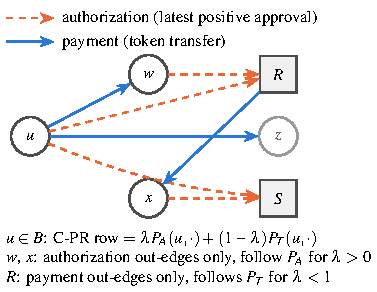
\includegraphics[width=\columnwidth]{figures/fig_layers.pdf}
\caption{The two layers on one set of addresses (schematic). Circles are sampled traders and squares are contracts such as routers and vaults; $z$ is an address outside the sample, present only because a sampled trader paid it. Only $u$ has out-edges in both layers, so only its row depends on $\lambda$ for $0<\lambda<1$. At $\lambda=1$ the payment edges and $z$ are dropped, so $R$ becomes dangling; at $\lambda=0$ the authorization edges are dropped, so $w$ and $x$ become dangling and $S$ leaves the graph. \spr{} walks the solid edges only and restarts each jump in proportion to the authorization walk's score.}
\label{fig:layers}
\end{figure}
